\texttt{Танцующие слоны}~--- это зрелищное шоу в Паттайе, в котором участвуют $N$ слонов, танцующих на одной линии, называемой \texttt{сценой}.

В результате многолетних тренировок слоны, участвующие в шоу, разучили большое количество танцевальных движений. Все шоу состоит из последовательности актов. В каждом акте только один слон совершает одно танцевальное движение, в результате которого он может переместиться на другую позицию на сцене.

Постановщики шоу хотят сделать фотоальбом, который бы содержал фотографии всего шоу. После каждого акта они хотят сделать фотографии всех слонов.

В любой момент времени на протяжении шоу некоторое количество слонов может находиться в одной и той же позиции~--- это значит, что слоны просто стоят рядом.

Одна фотокамера может фотографировать группу слонов тогда и только тогда, когда все позиции, в которых находятся слоны, лежат на отрезке длины $L$ (обе границы отрезка включаются в него). Так как слоны могут располагаться вдоль всей сцены, то может потребоваться несколько фотокамер, чтобы сфотографировать всех слонов одновременно.

К примеру, предположим, что $L=10$ и слоны располагаются на сцене в позициях $10$, $15$, $17$, и $20$ соответственно. В этот момент достаточно одной фотокамеры, чтобы сфотографировать всех слонов, как это показано ниже. (Слоны изображены как треугольники; фотокамеры изображены как трапеции).

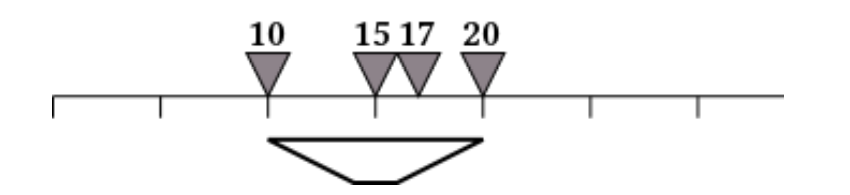
\includegraphics{elephants3.png}

В последующем акте слон, находящийся в позиции $15$, в результате танцевального движения перемещается в позицию $32$. После этого акта необходимо уже не менее двух фотокамер для того, чтобы сфотографировать всех слонов одновременно.

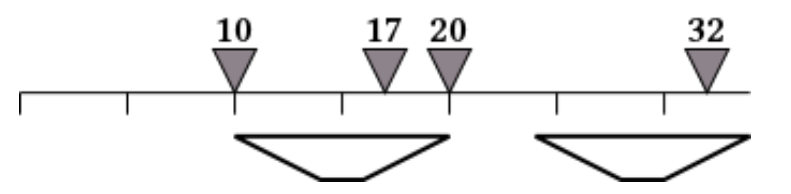
\includegraphics{elephants2.png}

В следующем акте слон, находящийся в позиции $10$, перемещается в позицию $7$. В данном случае понадобится 3 фотокамеры для того, чтобы сфотографировать всех слонов.

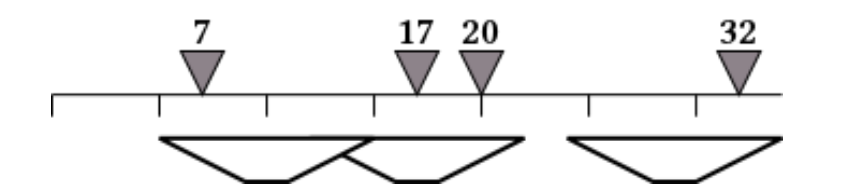
\includegraphics{elephants1.png}

В данной задаче, которая является интерактивной, вы должны определить минимальное количество фотокамер, необходимых для того, чтобы сделать фотографии после каждого акта шоу. Следует отметить, что количество необходимых фотокамер может увеличиваться, уменьшаться, или оставаться тем же самым от акта к акту.


Реализуйте:
\begin{itemize}

\item Процедуру \t{init(N,L,X)}, которой передаются следующие параметры:
\begin{itemize}
\item $N$~--- количество слонов. Слоны нумеруются от $0$ до $N-1$.

\item $L$~--- Длина отрезка, охватываемого одной фотокамерой. Гарантируется, что целое число $L$ удовлетворяет ограничению: $0 \le L \le 1\,000\,000\,000$.

\item $X$~--- одномерный массив целых чисел, представляющий собой начальные позиции слонов. Для каждого $0 \le i < N$ слон с номером $i$ находится в позиции $X[i]$. Начальные позиции упорядочены. Точнее, гарантируется, что $0 \le X[0] \le \dots \le X[N-1] \le 1\,000\,000\,000$. Следует отметить, что в течение танца при изменении позиции слонов может изменяться и порядок их следования.

\end{itemize}

Эта процедура будет вызвана ровно один раз (до всех вызовов процедуры \t{update}). Эта процедура не возвращает никакого значения.
\item Процедуру \t{update(i,y)}, которой передаются следующие параметры:
\begin{itemize}
\item $i$~--- номер слона, который передвигается в данном акте.
\item $y$~--- позиция, в которой слон с номером $i$ будет стоять после данного акта. Гарантируется, что целое число $y$ удовлетворяет ограничению: $0 \le y \le 1\,000\,000\,000$.
\end{itemize}
Данная процедура будет вызываться много раз. Каждый вызов соответствует одному акту, который находится в последовательности актов после всех предыдущих актов, для которых ранее вызывалась процедура. Каждый вызов должен вернуть минимальное количество фотокамер, необходимых для фотографирования после соответствующего акта.
\end{itemize}


